%% AMS-LaTeX Created with the Wolfram Language : www.wolfram.com

\documentclass[12pt]{article}

\usepackage[letterpaper,margin=1in]{geometry}
\usepackage{amsmath,amssymb,setspace}
\usepackage{graphicx}
\usepackage{bm}
\graphicspath{{./figs/}}
\usepackage{tcolorbox}
\usepackage[framed,numbered,autolinebreaks,useliterate]{mcode}
\usepackage{enumitem}
\usepackage{xcolor}
\usepackage{listings}
\usepackage{hyperref}
\usepackage[cal=boondox]{mathalfa}
\usepackage{tikz}
\usetikzlibrary{positioning}

% Define colors for lstlisting
\definecolor{codegreen}{rgb}{0,0.6,0}
\definecolor{codegray}{rgb}{0.5,0.5,0.5}
\definecolor{codepurple}{rgb}{0.58,0,0.82}
\definecolor{backcolour}{rgb}{0.95,0.95,0.95}

\lstdefinestyle{mystyle}{
    backgroundcolor=\color{backcolour},   
    commentstyle=\color{codegreen},
    keywordstyle=\color{magenta},
    numberstyle=\tiny\color{codegray},
    stringstyle=\color{codepurple},
    basicstyle=\ttfamily\normalsize,
    breakatwhitespace=false,         
    breaklines=true,                 
    captionpos=b,                    
    keepspaces=true,                 
    numbers=none,  
    columns=flexible,         
    numbersep=5pt,                  
    showspaces=false,                
    showstringspaces=false,
    showtabs=false,                  
    tabsize=2,
    literate={'}{{\textquotesingle}}1 {''}{{\textquotedbl}}2
}
\lstset{style=mystyle}

\hypersetup{
    colorlinks=true,
    linkcolor=blue,
    filecolor=magenta,      
    urlcolor=cyan,
    pdftitle={Your Document Title},
    pdfpagemode=FullScreen,
}

\def\mathbi#1{\textbf{\em #1}}
\newcommand{\fullunderline}{\noindent\makebox[\linewidth]{\rule{\linewidth}{0.1pt}}\\[-2em]}

\begin{document}
\doublespacing	

\title{CE 401/5501 Homework 06\\[2in]
\textbf{Name: \rule{2in}{0.15mm}}}
\author{}
\date{}
\maketitle

\newcommand*{\I}{\imath} % imaginary unit i

\newpage

\section{Multiple Choice / Fill-in-the-blank Questions}

\textbf{Question 1} \\

A perceptron is the simplest artificial neural network, and its mathematical expression can be written as 
\[
y = f\big[u(\bm{x})\big],
\]
where \( u(\bm{x}) = \bm{w}^T \bm{x} + b \). Which of the following statements describes its architecture? 

\begin{itemize}
    \item [$\checkmark$] The functional model describes a computing flow: Input features \(\bm{x}\) \(\rightarrow\) aggregation through \(u(\cdot)\) \(\rightarrow\) activation through \(f(\cdot)\) \(\rightarrow\) outputting a class label or score \(y\).
    \item [$\checkmark$] \(f(\cdot)\) is called an activation function, which is often a simple nonlinear function.
    \item [$\square$] The perceptron model is equivalent to a logistic regression model.
    \item [$\square$] The output \(y\) must be binary.
\end{itemize}

\bigskip

\newpage 

\textbf{Question 2} \\

Given a perceptron model for binary classification, its input is a two-dimensional data point denoted by 
\[
\bm{x} = \begin{bmatrix} x_1 \\ x_2 \end{bmatrix}.
\]
After learning from the data, the resulting learned weights and bias are 
\[
[w_1, w_2, b]^T = [-4, -3, 10]^T.
\]
Answer the following analysis questions:

\begin{itemize}
    \item Write down the decision function \( u(\bm{x}) \).  
    \textbf{Answer}: \( u(\bm{x}) = -4x_1 - 3x_2 + 10 \)
    \item In the \(x_1\text{-}x_2\) plane, plot the decision boundary \( u(\bm{x}) = 0 \) (hint: write it as \(x_2\) as a function of \(x_1\)).  
    \textbf{Answer}: \( -4x_1 - 3x_2 + 10 = 0 \implies x_2 = -\frac{4}{3}x_1 + \frac{10}{3} \)  
    (The plot is a line with slope \(-\frac{4}{3}\) and y-intercept \(\frac{10}{3}\).)
    \item Given that the activation is a \textit{Heaviside} function, write out the resulting perceptron model.  
    \textbf{Answer}: \( y = f(u(\bm{x})) = \begin{cases} 1 & \text{if } -4x_1 - 3x_2 + 10 \geq 0 \\ 0 & \text{otherwise} \end{cases} \)
    \item Given two data points:
    \begin{itemize}
        \item A: \([1, 4]^T\)
        \item B: \([-2, 2]^T\)
    \end{itemize}
    Using the perceptron model, Point A will be labeled as \textbf{(0)}; and Point B will be labeled as \textbf{(1)}.
    \item If the activation is a \textit{ReLU} function:
    \begin{itemize}
        \item For Point A: \([1, 4]^T\), the predicted score is \textbf{(0)}.
        \item For Point B: \([-2, 2]^T\), the predicted score is \textbf{(12)}.
    \end{itemize}
\end{itemize}

\bigskip

\newpage

\textbf{Question 3} \\

Suppose that a civil engineer is constructing an ML exercise. The input data point is 3-dimensional; namely, each data point is expressed as a \(3\times 1\) vector. There are two class labels, 0 and 1. The engineer has collected 1000 data points and manually labeled them.

The engineer starts with an initial neural network and configures it as follows:
\begin{itemize}
    \item The neural network has two hidden layers. Each hidden layer contains 5 neurons.
    \item The engineer's next task is to determine how many parameters (weights) the NN model has, assuming it is a fully connected multilayer perceptron. Here, we consider bias (intercept) parameters at each layer. Effectively, there is an additional input of 1 at each layer (the input layer and the two hidden layers).
\end{itemize}
Now you are tasked to answer:
\begin{itemize}
    \item How many weight parameters are in the model?  
    \textbf{Answer}:  
    - Input to Hidden 1: \( 4 \times 5 = 20 \) (3 features + 1 bias, 5 neurons).  
    - Hidden 1 to Hidden 2: \( 6 \times 5 = 30 \) (5 neurons + 1 bias, 5 neurons).  
    - Hidden 2 to Output: \( 6 \times 1 = 6 \) (5 neurons + 1 bias, 1 neuron).  
    - Total: \( 20 + 30 + 6 = 56 \).
    \item Graph the MLP neural network.  
    \textbf{Answer}: See the diagram below:  
\usetikzlibrary{positioning}

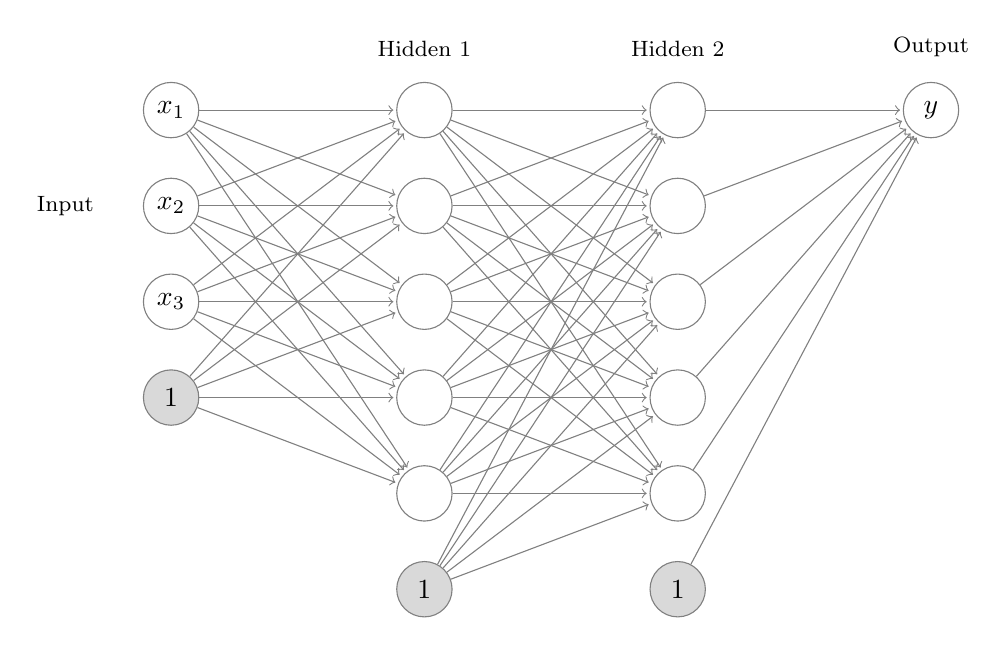
\begin{tikzpicture}[shorten >=1pt,->,draw=black!50, node distance=2.5cm]
    \tikzstyle{neuron}=[circle, draw, fill=white, minimum size=20pt, inner sep=0pt]
    \tikzstyle{bias}=[circle, draw, fill=gray!30, minimum size=20pt, inner sep=0pt]
    \tikzstyle{label}=[font=\footnotesize]

    % Input layer (3 features + 1 bias)
    \node[neuron] (I1) {$x_1$};
    \node[neuron, below=0.5cm of I1] (I2) {$x_2$};
    \node[neuron, below=0.5cm of I2] (I3) {$x_3$};
    \node[bias, below=0.5cm of I3] (IB) {$1$};
    \node[label, left=0.5cm of I2] {Input};

    % Hidden layer 1 (5 neurons + 1 bias)
    \node[neuron, right=2.5cm of I1] (H11) {};
    \node[neuron, below=0.5cm of H11] (H12) {};
    \node[neuron, below=0.5cm of H12] (H13) {};
    \node[neuron, below=0.5cm of H13] (H14) {};
    \node[neuron, below=0.5cm of H14] (H15) {};
    \node[bias, below=0.5cm of H15] (H1B) {$1$};
    \node[label, above=0.2cm of H11] {Hidden 1};

    % Hidden layer 2 (5 neurons + 1 bias)
    \node[neuron, right=2.5cm of H11] (H21) {};
    \node[neuron, below=0.5cm of H21] (H22) {};
    \node[neuron, below=0.5cm of H22] (H23) {};
    \node[neuron, below=0.5cm of H23] (H24) {};
    \node[neuron, below=0.5cm of H24] (H25) {};
    \node[bias, below=0.5cm of H25] (H2B) {$1$};
    \node[label, above=0.2cm of H21] {Hidden 2};

    % Output layer (1 neuron)
    \node[neuron, right=2.5cm of H21] (O1) {$y$};
    \node[label, above=0.2cm of O1] {Output};

    % Connections
    % Input to Hidden 1 (bias IB connects only to H11-H15, not H1B)
    \foreach \i in {1,2,3}
        \foreach \j in {1,2,3,4,5}
            \draw (I\i) -- (H1\j);
    \foreach \j in {1,2,3,4,5}
        \draw (IB) -- (H1\j);

    % Hidden 1 to Hidden 2 (bias H1B connects only to H21-H25, not H2B)
    \foreach \i in {1,2,3,4,5}
        \foreach \j in {1,2,3,4,5}
            \draw (H1\i) -- (H2\j);
    \foreach \j in {1,2,3,4,5}
        \draw (H1B) -- (H2\j);

    % Hidden 2 to Output (bias H2B connects only to O1)
    \foreach \i in {1,2,3,4,5}
        \draw (H2\i) -- (O1);
    \draw (H2B) -- (O1);
\end{tikzpicture}

\end{itemize}

\newpage

\end{document}